% Document setup
\documentclass[11pt]{book}

% Location of the csas-style repository: adjust path as needed
\newcommand{\locRepo}{csas-style}

% Use the style file in the csas-style repository (sr.sty)
\usepackage{\locRepo/sr}

% header-includes from R markdown entry
\usepackage{pdflscape}

% Bibliography style file
% \bibliographystyle{../csas-style/res-doc}

%%%% Commands for title page etc %%%%%

% Title
\newcommand{\rdTitle}{Evaluating the robustness of candidate management procedures in the BC sablefish (\emph{Anoplopoma fibria}) for 2019-2020.}

% French title
\newcommand{\rdTitleFr}{}

% Title short
\newcommand{\rdTitleShort}{Robustness of sablefish MPs in BC}

% Publication year
\newcommand{\rdYear}{2019}

% Publication month
\newcommand{\rdMonth}{October}

% Report number
\newcommand{\rdNumber}{nnn}

% Approver (name\\position)
\newcommand{\rdApp}{Approver Name\\
Regional Director\\
Science Branch, Pacific Region\\
Fisheries and Oceans Canada}
% \newcommand{\rdYear}{20XX}
% \newcommand{\rdAppMonth}{January}
% \newcommand{\rdAppDay}{01}
\newcommand{\rdAppDate}{January 01, 20XX}

% Branch
\newcommand{\rdBranch}{Science Branch}

% Region
\newcommand{\rdRegion}{Pacific Region}

% Address
\newcommand{\rdAddress}{\textsuperscript{1}Pacific Biological Station\\
Fisheries and Oceans Canada, 3190 Hammond Bay Road\\
Nanaimo, British Columbia, V9T 6N7, Canada\\
\textsuperscript{2}Far, far away\\
Another Galaxy}

% Phone
\newcommand{\rdPhone}{(250) 756-7208}

% Email
\newcommand{\rdEmail}{\href{mailto:csap@dfo-mpo.gc.ca}{\nolinkurl{csap@dfo-mpo.gc.ca}}}

%%%% End of title page commands %%%%%
\begin{document}

\MakeFirstPage

\newpage

\hypertarget{tables}{%
\section{Tables}\label{tables}}

\newpage

\begingroup\fontsize{12}{14}\selectfont
\begin{landscape}
\begin{longtable}[t]{llllllll}
\caption{\label{tab:unnamed-chunk-3}Operating model posterior mean (standard deviation) biological parameter and reference point estimates for the full posterior and 5 sampled regions for each productivity/biomass scenario.}\\
\toprule
\textbf{ } & \textbf{2016 Fit} & \textbf{2018 Fit} & \textbf{hiB} & \textbf{hih} & \textbf{loB} & \textbf{loh} & \textbf{mhmB}\\
\midrule
\endfirsthead
\caption*{}\\
\toprule
\textbf{ } & \textbf{2016 Fit} & \textbf{2018 Fit} & \textbf{hiB} & \textbf{hih} & \textbf{loB} & \textbf{loh} & \textbf{mhmB}\\
\midrule
\endhead
\
\endfoot
\bottomrule
\endlastfoot
$B_0$ & 57 (1.3) & 54.1 (3.3) & 55.6 & 53.9 & 52.2 & 54.2 & 54\\
$M_m$ & 0.0411 (0.00027) & 0.0421 (0.0026) & 0.0425 & 0.0419 & 0.0412 & 0.0422 & 0.042\\
$M_f$ & 0.0788 (0.0014) & 0.0877 (0.0025) & 0.087 & 0.0874 & 0.0879 & 0.0879 & 0.0876\\
$h$ & 0.556 (0.064) & 0.617 (0.062) & 0.62 & 0.689 & 0.617 & 0.545 & 0.618\\
$B_{2016}$ & 10.9 (1.2) & 12.5 (1.4) & 14 & 12.4 & 11 & 12.5 & 12.5\\
$B_{2018}$ &  & 16.3 (2) & 18.6 & 16.2 & 14.1 & 16.4 & 16.3\\
$B_{MSY}$ & 23.4 (0.96) & 20.4 (1.7) & 20.9 & 18.9 & 19.8 & 21.9 & 20.4\\
$U_{MSY}$ & 0.0433 (0.0062) & 0.0734 (0.01) & 0.0736 & 0.0853 & 0.0729 & 0.0619 & 0.0733\\
Legal $U_{MSY}$ & 0.0423 (0.006) & 0.0773 (0.011) & 0.0775 & 0.0902 & 0.0766 & 0.0647 & 0.0771\\
$MSY$ & 2.79 (0.27) & 4.37 (0.45) & 4.46 & 4.75 & 4.27 & 3.98 & 4.38\\
$B_{2016}/B_0$ & 0.191 (0.018) & 0.231 (0.021) & 0.253 & 0.231 & 0.212 & 0.232 & 0.231\\
$B_{2016}/B_{MSY}$ & 0.467 (0.049) & 0.613 (0.065) & 0.673 & 0.66 & 0.558 & 0.573 & 0.612\\
$B_{2018}/B_0$ &  & 0.301 (0.032) & 0.335 & 0.301 & 0.271 & 0.304 & 0.302\\
$B_{2018}/B_{MSY}$ &  & 0.8 (0.096) & 0.891 & 0.86 & 0.714 & 0.75 & 0.799\\*
\end{longtable}
\end{landscape}
\endgroup{}

\newpage

\begingroup\fontsize{9}{11}\selectfont
\begin{landscape}
\begin{longtable}[t]{llccccccccc}
\caption{\label{tab:unnamed-chunk-5}Weighted performance metrics for all candidate management procedures on the reference set of operating models, where recruitment is taken from the OM estimate in 2016. Conservation performance metrics that pass the criteria in the header are indicated by a bullet.}\\
\toprule
\multicolumn{2}{c}{\textbf{ }} & \multicolumn{1}{c}{\textbf{Objective 1}} & \multicolumn{1}{c}{\textbf{Objective 2}} & \multicolumn{1}{c}{\textbf{Objective 3}} & \multicolumn{1}{c}{\textbf{Objective 4}} & \multicolumn{1}{c}{\textbf{Objective 5}} & \multicolumn{4}{c}{\textbf{Other Important Quantities}} \\
\cmidrule(l{3pt}r{3pt}){3-3} \cmidrule(l{3pt}r{3pt}){4-4} \cmidrule(l{3pt}r{3pt}){5-5} \cmidrule(l{3pt}r{3pt}){6-6} \cmidrule(l{3pt}r{3pt}){7-7} \cmidrule(l{3pt}r{3pt}){8-11}
\multicolumn{2}{c}{\textbf{ }} & \multicolumn{1}{c}{\textbf{P > .95}} & \multicolumn{1}{c}{\textbf{Obs < Acc}} & \multicolumn{1}{c}{\textbf{P > .5}} & \multicolumn{1}{c}{\textbf{min}} & \multicolumn{1}{c}{\textbf{max}} & \multicolumn{4}{c}{\textbf{ }} \\
\cmidrule(l{3pt}r{3pt}){3-3} \cmidrule(l{3pt}r{3pt}){4-4} \cmidrule(l{3pt}r{3pt}){5-5} \cmidrule(l{3pt}r{3pt}){6-6} \cmidrule(l{3pt}r{3pt}){7-7}
\textbf{No.} & \textbf{MP Label} & \textbf{$P(B_t \geq .4B_{MSY})$} & \textbf{$P(Decline)$} & \textbf{$P(B_{2052} > B_{MSY})$} & \textbf{$P(C_t < 1.992)$} & \textbf{$\bar{C}_{2019:2028}$} & \textbf{$AAV$} & \textbf{$C_{2019}$} & \textbf{$D_{2019}$} & \textbf{$F_{2022}$}\\
\midrule
\endfirsthead
\caption*{}\\
\toprule
\textbf{No.} & \textbf{MP Label} & \textbf{$P(B_t \geq .4B_{MSY})$} & \textbf{$P(Decline)$} & \textbf{$P(B_{2052} > B_{MSY})$} & \textbf{$P(C_t < 1.992)$} & \textbf{$\bar{C}_{2019:2028}$} & \textbf{$AAV$} & \textbf{$C_{2019}$} & \textbf{$D_{2019}$} & \textbf{$F_{2022}$}\\
\midrule
\endhead
\
\endfoot
\bottomrule
\endlastfoot
14 & frt & $\bullet$ & $\bullet$ & $\bullet$ & 0.0148 & 4.51 & 7.81 & 3.39 & 0.353 & 0.0738\\
3 & cap.5\_hstAl\_am5 & $\bullet$ & $\bullet$ & $\bullet$ & 0.0217 & 4.01 & 8.01 & 3.39 & 0.353 & 0.0728\\
5 & cap.5\_rctAl\_am5 & $\bullet$ & $\bullet$ & $\bullet$ & 0.0217 & 3.93 & 7.95 & 3.39 & 0.353 & 0.0712\\
7 & cap1.0\_hstAl\_am5 & $\bullet$ & $\bullet$ & $\bullet$ & 0.0217 & 3.93 & 8.07 & 3.39 & 0.353 & 0.0680\\
2 & cap.5\_hstAl\_am10 & $\bullet$ & $\bullet$ & $\bullet$ & 0.0217 & 3.92 & 7.99 & 3.39 & 0.353 & 0.0665\\
4 & cap.5\_rctAl\_am10 & $\bullet$ & $\bullet$ & $\bullet$ & 0.0232 & 3.86 & 8.10 & 3.39 & 0.353 & 0.0654\\
6 & cap1.0\_hstAl\_am10 & $\bullet$ & $\bullet$ & $\bullet$ & 0.0217 & 3.85 & 8.23 & 3.39 & 0.353 & 0.0636\\
11 & cap1.5\_hstAl\_am5 & $\bullet$ & $\bullet$ & $\bullet$ & 0.0232 & 3.84 & 8.34 & 3.39 & 0.353 & 0.0638\\
10 & cap1.5\_hstAl\_am10 & $\bullet$ & $\bullet$ & $\bullet$ & 0.0232 & 3.80 & 8.03 & 3.39 & 0.353 & 0.0613\\
8 & cap1.0\_rctAl\_am10 & $\bullet$ & $\bullet$ & $\bullet$ & 0.0265 & 3.78 & 8.18 & 3.39 & 0.353 & 0.0624\\
9 & cap1.0\_rctAl\_am5 & $\bullet$ & $\bullet$ & $\bullet$ & 0.0232 & 3.77 & 8.17 & 3.39 & 0.353 & 0.0651\\
15 & noCap & $\bullet$ & $\bullet$ & $\bullet$ & 0.0265 & 3.73 & 7.02 & 3.39 & 0.353 & 0.0582\\
12 & cap1.5\_rctAl\_am10 & $\bullet$ & $\bullet$ & $\bullet$ & 0.0265 & 3.72 & 8.26 & 3.39 & 0.353 & 0.0603\\
13 & cap1.5\_rctAl\_am5 & $\bullet$ & $\bullet$ & $\bullet$ & 0.0232 & 3.70 & 8.37 & 3.39 & 0.353 & 0.0621\\
1 & NoFish & $\bullet$ & $\bullet$ & $\bullet$ & 1.0000 & 0.00 & 0.00 & 0.00 & 0.353 & 0.0550\\*
\end{longtable}
\end{landscape}
\endgroup{}

\newpage

\begingroup\fontsize{9}{11}\selectfont
\begin{landscape}
\begin{longtable}[t]{llccccccccc}
\caption{\label{tab:unnamed-chunk-6}Weighted performance metrics for all candidate management procedures on the robustness set of operating models, where recruitment is simulated stochastically off the stock-recruit curve in 2016. Conservation performance metrics that pass the criteria in the header are indicated by a bullet.}\\
\toprule
\multicolumn{2}{c}{\textbf{ }} & \multicolumn{1}{c}{\textbf{Objective 1}} & \multicolumn{1}{c}{\textbf{Objective 2}} & \multicolumn{1}{c}{\textbf{Objective 3}} & \multicolumn{1}{c}{\textbf{Objective 4}} & \multicolumn{1}{c}{\textbf{Objective 5}} & \multicolumn{4}{c}{\textbf{Other Important Quantities}} \\
\cmidrule(l{3pt}r{3pt}){3-3} \cmidrule(l{3pt}r{3pt}){4-4} \cmidrule(l{3pt}r{3pt}){5-5} \cmidrule(l{3pt}r{3pt}){6-6} \cmidrule(l{3pt}r{3pt}){7-7} \cmidrule(l{3pt}r{3pt}){8-11}
\multicolumn{2}{c}{\textbf{ }} & \multicolumn{1}{c}{\textbf{P > .95}} & \multicolumn{1}{c}{\textbf{Obs < Acc}} & \multicolumn{1}{c}{\textbf{P > .5}} & \multicolumn{1}{c}{\textbf{min}} & \multicolumn{1}{c}{\textbf{max}} & \multicolumn{4}{c}{\textbf{ }} \\
\cmidrule(l{3pt}r{3pt}){3-3} \cmidrule(l{3pt}r{3pt}){4-4} \cmidrule(l{3pt}r{3pt}){5-5} \cmidrule(l{3pt}r{3pt}){6-6} \cmidrule(l{3pt}r{3pt}){7-7}
\textbf{No.} & \textbf{MP Label} & \textbf{$P(B_t \geq .4B_{MSY})$} & \textbf{$P(Decline)$} & \textbf{$P(B_{2052} > B_{MSY})$} & \textbf{$P(C_t < 1.992)$} & \textbf{$\bar{C}_{2019:2028}$} & \textbf{$AAV$} & \textbf{$C_{2019}$} & \textbf{$D_{2019}$} & \textbf{$F_{2022}$}\\
\midrule
\endfirsthead
\caption*{}\\
\toprule
\textbf{No.} & \textbf{MP Label} & \textbf{$P(B_t \geq .4B_{MSY})$} & \textbf{$P(Decline)$} & \textbf{$P(B_{2052} > B_{MSY})$} & \textbf{$P(C_t < 1.992)$} & \textbf{$\bar{C}_{2019:2028}$} & \textbf{$AAV$} & \textbf{$C_{2019}$} & \textbf{$D_{2019}$} & \textbf{$F_{2022}$}\\
\midrule
\endhead
\
\endfoot
\bottomrule
\endlastfoot
14 & frt & $\bullet$ & $\bullet$ & $\bullet$ & 0.0798 & 2.77 & 11.2 & 3.39 & 0.24 & 0.0674\\
3 & cap.5\_hstAl\_am5 & $\bullet$ & $\bullet$ & $\bullet$ & 0.1750 & 2.44 & 14.8 & 3.40 & 0.24 & 0.0643\\
7 & cap1.0\_hstAl\_am5 & $\bullet$ & $0.267>0.263$ & $\bullet$ & 0.2030 & 2.39 & 14.8 & 3.40 & 0.24 & 0.0589\\
2 & cap.5\_hstAl\_am10 & $\bullet$ & $\bullet$ & $\bullet$ & 0.2050 & 2.39 & 15.0 & 3.40 & 0.24 & 0.0592\\
5 & cap.5\_rctAl\_am5 & $\bullet$ & $\bullet$ & $\bullet$ & 0.2120 & 2.38 & 15.3 & 3.40 & 0.24 & 0.0622\\
6 & cap1.0\_hstAl\_am10 & $\bullet$ & $\bullet$ & $\bullet$ & 0.2220 & 2.36 & 14.9 & 3.40 & 0.24 & 0.0564\\
11 & cap1.5\_hstAl\_am5 & $\bullet$ & $0.272>0.263$ & $\bullet$ & 0.2230 & 2.36 & 14.5 & 3.40 & 0.24 & 0.0556\\
4 & cap.5\_rctAl\_am10 & $\bullet$ & $\bullet$ & $\bullet$ & 0.2280 & 2.35 & 15.3 & 3.40 & 0.24 & 0.0580\\
10 & cap1.5\_hstAl\_am10 & $\bullet$ & $\bullet$ & $\bullet$ & 0.2380 & 2.34 & 14.3 & 3.40 & 0.24 & 0.0543\\
12 & cap1.5\_rctAl\_am10 & $\bullet$ & $\bullet$ & $\bullet$ & 0.2440 & 2.32 & 14.6 & 3.40 & 0.24 & 0.0540\\
8 & cap1.0\_rctAl\_am10 & $\bullet$ & $\bullet$ & $\bullet$ & 0.2380 & 2.32 & 15.3 & 3.40 & 0.24 & 0.0552\\
13 & cap1.5\_rctAl\_am5 & $\bullet$ & $\bullet$ & $\bullet$ & 0.2400 & 2.31 & 15.2 & 3.40 & 0.24 & 0.0546\\
9 & cap1.0\_rctAl\_am5 & $\bullet$ & $\bullet$ & $\bullet$ & 0.2430 & 2.31 & 15.7 & 3.40 & 0.24 & 0.0567\\
15 & noCap & $\bullet$ & $\bullet$ & $\bullet$ & 0.2540 & 2.31 & 14.2 & 3.40 & 0.24 & 0.0524\\
1 & NoFish & $\bullet$ & $\bullet$ & $\bullet$ & 1.0000 & 0.00 & 0.0 & 0.00 & 0.24 & 0.0550\\*
\end{longtable}
\end{landscape}
\endgroup{}

\newpage

\begingroup\fontsize{12}{14}\selectfont
\begin{landscape}
\begin{longtable}[t]{llcccccccccl}
\caption{\label{tab:unnamed-chunk-7}Weighted economic performance metrics for the first 10 years of the projections in the reference OM set. Column 3 shows the average catch over the first 10 years, and the remaining columns show the total value (\$m) of catch $C$ and discards $D$ for all sectors, and the yearly average income $I$ in dollars per tonne of catch, over the next 10 years. All values are taken at 4 significant figures.}\\
\toprule
\multicolumn{2}{c}{\textbf{ }} & \multicolumn{1}{c}{\textbf{Av. Catch (kt)}} & \multicolumn{6}{c}{\textbf{10 year value (\$ millions)}} & \multicolumn{3}{c}{\textbf{Av. income (\$/t)}} \\
\cmidrule(l{3pt}r{3pt}){3-3} \cmidrule(l{3pt}r{3pt}){4-9} \cmidrule(l{3pt}r{3pt}){10-12}
\textbf{No.} & \textbf{MP Label} & \textbf{$\bar{C}_{2019:2028}$} & \textbf{$C^{trap}$} & \textbf{$C^{hook}$} & \textbf{$C^{trawl}$} & \textbf{$D^{trap}$} & \textbf{$D^{hook}$} & \textbf{$D^{trawl}$} & \textbf{$I^{trap}$} & \textbf{$I^{hook}$} & \textbf{$I^{trawl}$}\\
\midrule
\endfirsthead
\caption*{}\\
\toprule
\textbf{No.} & \textbf{MP Label} & \textbf{$\bar{C}_{2019:2028}$} & \textbf{$C^{trap}$} & \textbf{$C^{hook}$} & \textbf{$C^{trawl}$} & \textbf{$D^{trap}$} & \textbf{$D^{hook}$} & \textbf{$D^{trawl}$} & \textbf{$I^{trap}$} & \textbf{$I^{hook}$} & \textbf{$I^{trawl}$}\\
\midrule
\endhead
\
\endfoot
\bottomrule
\endlastfoot
14 & frt & 4.510 & 417.6 & 335.4 & 60.81 & 0.000 & 0.00 & 0.00 & 17970 & 18320 & 16270\\
3 & cap.5\_hstAl\_am5 & 4.005 & 370.9 & 312.5 & 46.34 & 10.550 & 13.08 & 27.75 & 18130 & 18340 & 17330\\
5 & cap.5\_rctAl\_am5 & 3.930 & 362.8 & 302.2 & 50.54 & 10.320 & 12.65 & 29.97 & 18140 & 18340 & 17330\\
7 & cap1.0\_hstAl\_am5 & 3.927 & 358.3 & 305.8 & 50.07 & 10.210 & 12.78 & 29.71 & 18140 & 18340 & 17330\\
2 & cap.5\_hstAl\_am10 & 3.921 & 364.1 & 299.3 & 49.78 & 10.400 & 12.53 & 29.86 & 18130 & 18340 & 17330\\
4 & cap.5\_rctAl\_am10 & 3.864 & 358.6 & 292.9 & 52.15 & 10.240 & 12.27 & 31.12 & 18140 & 18340 & 17340\\
6 & cap1.0\_hstAl\_am10 & 3.850 & 355.3 & 294.0 & 51.77 & 10.160 & 12.31 & 30.90 & 18140 & 18340 & 17340\\
11 & cap1.5\_hstAl\_am5 & 3.842 & 348.0 & 298.1 & 52.75 & 9.943 & 12.46 & 31.14 & 18140 & 18340 & 17340\\
10 & cap1.5\_hstAl\_am10 & 3.804 & 349.1 & 289.1 & 53.25 & 10.000 & 12.11 & 31.70 & 18140 & 18340 & 17340\\
8 & cap1.0\_rctAl\_am10 & 3.782 & 348.5 & 284.7 & 55.07 & 9.982 & 11.93 & 32.71 & 18140 & 18340 & 17340\\
9 & cap1.0\_rctAl\_am5 & 3.767 & 343.6 & 286.5 & 55.58 & 9.818 & 12.00 & 32.67 & 18140 & 18340 & 17340\\
15 & noCap & 3.729 & 347.9 & 277.5 & 53.58 & 10.010 & 11.66 & 32.11 & 18140 & 18340 & 17340\\
12 & cap1.5\_rctAl\_am10 & 3.721 & 342.4 & 279.8 & 54.97 & 9.830 & 11.73 & 32.73 & 18140 & 18340 & 17340\\
13 & cap1.5\_rctAl\_am5 & 3.702 & 336.7 & 280.8 & 56.10 & 9.642 & 11.76 & 33.18 & 18140 & 18340 & 17340\\
1 & NoFish & 0.000 & 0.0 & 0.0 & 0.00 & 0.000 & 0.00 & 0.00 & 0 & 0 & 0\\*
\end{longtable}
\end{landscape}
\endgroup{}

\newpage

\begingroup\fontsize{12}{14}\selectfont
\begin{landscape}
\begin{longtable}[t]{llcccccccccl}
\caption{\label{tab:unnamed-chunk-8}Weighted economic performance metrics for the first 10 years of the projections in the reference OM set. Column 3 shows the average catch over the first 10 years, and the remaining columns show the total value (\$m) of catch $C$ and discards $D$ for all sectors, and the yearly average income $I$ in dollars per tonne of catch, over the next 10 years. All values are taken at 4 significant figures.}\\
\toprule
\multicolumn{2}{c}{\textbf{ }} & \multicolumn{1}{c}{\textbf{Av. Catch (kt)}} & \multicolumn{6}{c}{\textbf{10 year value (\$ millions)}} & \multicolumn{3}{c}{\textbf{Av. income (\$/t)}} \\
\cmidrule(l{3pt}r{3pt}){3-3} \cmidrule(l{3pt}r{3pt}){4-9} \cmidrule(l{3pt}r{3pt}){10-12}
\textbf{No.} & \textbf{MP Label} & \textbf{$\bar{C}_{2019:2028}$} & \textbf{$C^{trap}$} & \textbf{$C^{hook}$} & \textbf{$C^{trawl}$} & \textbf{$D^{trap}$} & \textbf{$D^{hook}$} & \textbf{$D^{trawl}$} & \textbf{$I^{trap}$} & \textbf{$I^{hook}$} & \textbf{$I^{trawl}$}\\
\midrule
\endfirsthead
\caption*{}\\
\toprule
\textbf{No.} & \textbf{MP Label} & \textbf{$\bar{C}_{2019:2028}$} & \textbf{$C^{trap}$} & \textbf{$C^{hook}$} & \textbf{$C^{trawl}$} & \textbf{$D^{trap}$} & \textbf{$D^{hook}$} & \textbf{$D^{trawl}$} & \textbf{$I^{trap}$} & \textbf{$I^{hook}$} & \textbf{$I^{trawl}$}\\
\midrule
\endhead
\
\endfoot
\bottomrule
\endlastfoot
14 & frt & 2.767 & 256.2 & 205.8 & 36.44 & 0.000 & 0.000 & 0.00 & 18030 & 18340 & 15880\\
3 & cap.5\_hstAl\_am5 & 2.440 & 226.8 & 189.8 & 26.25 & 5.976 & 7.804 & 19.56 & 18200 & 18370 & 17220\\
7 & cap1.0\_hstAl\_am5 & 2.392 & 220.4 & 184.6 & 29.42 & 5.778 & 7.571 & 22.07 & 18200 & 18370 & 17230\\
2 & cap.5\_hstAl\_am10 & 2.385 & 223.0 & 182.3 & 28.56 & 5.853 & 7.482 & 21.69 & 18200 & 18370 & 17230\\
5 & cap.5\_rctAl\_am5 & 2.377 & 220.6 & 181.0 & 29.58 & 5.776 & 7.426 & 22.12 & 18200 & 18370 & 17230\\
6 & cap1.0\_hstAl\_am10 & 2.364 & 219.4 & 179.3 & 30.70 & 5.741 & 7.351 & 23.39 & 18200 & 18370 & 17240\\
11 & cap1.5\_hstAl\_am5 & 2.358 & 218.2 & 178.0 & 31.63 & 5.696 & 7.292 & 23.92 & 18200 & 18370 & 17240\\
4 & cap.5\_rctAl\_am10 & 2.349 & 219.3 & 177.4 & 30.72 & 5.735 & 7.274 & 23.37 & 18200 & 18370 & 17240\\
10 & cap1.5\_hstAl\_am10 & 2.340 & 217.2 & 175.1 & 32.03 & 5.670 & 7.176 & 24.50 & 18210 & 18370 & 17240\\
12 & cap1.5\_rctAl\_am10 & 2.322 & 214.6 & 173.2 & 33.28 & 5.590 & 7.083 & 25.58 & 18210 & 18370 & 17240\\
8 & cap1.0\_rctAl\_am10 & 2.322 & 215.0 & 173.8 & 33.06 & 5.605 & 7.114 & 25.30 & 18210 & 18370 & 17240\\
13 & cap1.5\_rctAl\_am5 & 2.312 & 212.5 & 173.4 & 33.49 & 5.526 & 7.091 & 25.62 & 18210 & 18370 & 17240\\
9 & cap1.0\_rctAl\_am5 & 2.309 & 212.7 & 174.3 & 33.22 & 5.537 & 7.131 & 25.16 & 18210 & 18370 & 17250\\
15 & noCap & 2.305 & 214.7 & 171.1 & 32.79 & 5.600 & 7.004 & 25.31 & 18210 & 18370 & 17240\\
1 & NoFish & 0.000 & 0.0 & 0.0 & 0.00 & 0.000 & 0.000 & 0.00 & 0 & 0 & 0\\*
\end{longtable}
\end{landscape}
\endgroup{}

\newpage

\begingroup\fontsize{9}{11}\selectfont
\begin{landscape}
\begin{longtable}[t]{llccccccccc}
\caption{\label{tab:unnamed-chunk-10}Weighted performance metrics for all candidate management procedures, with harvest rates tuned to performance on the reference set of operating models, and applied to the robustness set of operating models where recruitment is simulated stochastically off the stock-recruit curve in 2016. Conservation performance metrics that pass the criteria in the header are indicated by a bullet.}\\
\toprule
\multicolumn{2}{c}{\textbf{ }} & \multicolumn{1}{c}{\textbf{Objective 1}} & \multicolumn{1}{c}{\textbf{Objective 2}} & \multicolumn{1}{c}{\textbf{Objective 3}} & \multicolumn{1}{c}{\textbf{Objective 4}} & \multicolumn{1}{c}{\textbf{Objective 5}} & \multicolumn{4}{c}{\textbf{Other Important Quantities}} \\
\cmidrule(l{3pt}r{3pt}){3-3} \cmidrule(l{3pt}r{3pt}){4-4} \cmidrule(l{3pt}r{3pt}){5-5} \cmidrule(l{3pt}r{3pt}){6-6} \cmidrule(l{3pt}r{3pt}){7-7} \cmidrule(l{3pt}r{3pt}){8-11}
\multicolumn{2}{c}{\textbf{ }} & \multicolumn{1}{c}{\textbf{P > .95}} & \multicolumn{1}{c}{\textbf{Obs < Acc}} & \multicolumn{1}{c}{\textbf{P > .5}} & \multicolumn{1}{c}{\textbf{min}} & \multicolumn{1}{c}{\textbf{max}} & \multicolumn{4}{c}{\textbf{ }} \\
\cmidrule(l{3pt}r{3pt}){3-3} \cmidrule(l{3pt}r{3pt}){4-4} \cmidrule(l{3pt}r{3pt}){5-5} \cmidrule(l{3pt}r{3pt}){6-6} \cmidrule(l{3pt}r{3pt}){7-7}
\textbf{No.} & \textbf{MP Label} & \textbf{$P(B_t \geq .4B_{MSY})$} & \textbf{$P(Decline)$} & \textbf{$P(B_{2052} > B_{MSY})$} & \textbf{$P(C_t < 1.992)$} & \textbf{$\bar{C}_{2019:2028}$} & \textbf{$AAV$} & \textbf{$C_{2019}$} & \textbf{$D_{2019}$} & \textbf{$F_{2022}$}\\
\midrule
\endfirsthead
\caption*{}\\
\toprule
\textbf{No.} & \textbf{MP Label} & \textbf{$P(B_t \geq .4B_{MSY})$} & \textbf{$P(Decline)$} & \textbf{$P(B_{2052} > B_{MSY})$} & \textbf{$P(C_t < 1.992)$} & \textbf{$\bar{C}_{2019:2028}$} & \textbf{$AAV$} & \textbf{$C_{2019}$} & \textbf{$D_{2019}$} & \textbf{$F_{2022}$}\\
\midrule
\endhead
\
\endfoot
\bottomrule
\endlastfoot
14 & frt & $\bullet$ & $\bullet$ & $0.419<0.5$ & 0.0882 & 2.92 & 10.9 & 3.39 & 0.24 & 0.0738\\
3 & cap.5\_hstAl\_am5 & $\bullet$ & $0.324>0.263$ & $0.408<0.5$ & 0.1370 & 2.61 & 13.8 & 3.40 & 0.24 & 0.0728\\
7 & cap1.0\_hstAl\_am5 & $\bullet$ & $0.344>0.263$ & $0.4<0.5$ & 0.1470 & 2.59 & 13.7 & 3.40 & 0.24 & 0.0680\\
5 & cap.5\_rctAl\_am5 & $\bullet$ & $0.331>0.263$ & $0.402<0.5$ & 0.1580 & 2.56 & 14.0 & 3.40 & 0.24 & 0.0712\\
2 & cap.5\_hstAl\_am10 & $\bullet$ & $0.324>0.263$ & $0.422<0.5$ & 0.1530 & 2.55 & 13.9 & 3.40 & 0.24 & 0.0665\\
11 & cap1.5\_hstAl\_am5 & $\bullet$ & $0.35>0.263$ & $0.411<0.5$ & 0.1680 & 2.54 & 13.5 & 3.40 & 0.24 & 0.0638\\
6 & cap1.0\_hstAl\_am10 & $\bullet$ & $0.338>0.263$ & $0.422<0.5$ & 0.1700 & 2.53 & 13.9 & 3.40 & 0.24 & 0.0636\\
4 & cap.5\_rctAl\_am10 & $\bullet$ & $0.33>0.263$ & $0.424<0.5$ & 0.1770 & 2.52 & 14.0 & 3.40 & 0.24 & 0.0654\\
10 & cap1.5\_hstAl\_am10 & $\bullet$ & $0.336>0.263$ & $0.427<0.5$ & 0.1880 & 2.50 & 13.3 & 3.40 & 0.24 & 0.0613\\
9 & cap1.0\_rctAl\_am5 & $\bullet$ & $0.338>0.263$ & $0.413<0.5$ & 0.1800 & 2.49 & 14.3 & 3.40 & 0.24 & 0.0651\\
8 & cap1.0\_rctAl\_am10 & $\bullet$ & $0.339>0.263$ & $0.417<0.5$ & 0.1900 & 2.49 & 14.2 & 3.40 & 0.24 & 0.0624\\
13 & cap1.5\_rctAl\_am5 & $\bullet$ & $0.338>0.263$ & $0.413<0.5$ & 0.1880 & 2.48 & 14.1 & 3.40 & 0.24 & 0.0621\\
12 & cap1.5\_rctAl\_am10 & $\bullet$ & $0.331>0.263$ & $0.425<0.5$ & 0.2000 & 2.46 & 13.6 & 3.40 & 0.24 & 0.0603\\
15 & noCap & $\bullet$ & $0.325>0.263$ & $0.437<0.5$ & 0.2080 & 2.45 & 13.0 & 3.40 & 0.24 & 0.0582\\
1 & NoFish & $\bullet$ & $\bullet$ & $\bullet$ & 1.0000 & 0.00 & 0.0 & 0.00 & 0.24 & 0.0550\\*
\end{longtable}
\end{landscape}
\endgroup{}

\newpage

\begingroup\fontsize{9}{11}\selectfont
\begin{landscape}
\begin{longtable}[t]{llccccccccc}
\caption{\label{tab:unnamed-chunk-11}Weighted performance metrics for all candidate management procedures, with harvest rates tuned to performance on the robustness set of operating models, and applied to the reference set of operating models accepting the high 2016 year class. Conservation performance metrics that pass the criteria in the header are indicated by a bullet.}\\
\toprule
\multicolumn{2}{c}{\textbf{ }} & \multicolumn{1}{c}{\textbf{Objective 1}} & \multicolumn{1}{c}{\textbf{Objective 2}} & \multicolumn{1}{c}{\textbf{Objective 3}} & \multicolumn{1}{c}{\textbf{Objective 4}} & \multicolumn{1}{c}{\textbf{Objective 5}} & \multicolumn{4}{c}{\textbf{Other Important Quantities}} \\
\cmidrule(l{3pt}r{3pt}){3-3} \cmidrule(l{3pt}r{3pt}){4-4} \cmidrule(l{3pt}r{3pt}){5-5} \cmidrule(l{3pt}r{3pt}){6-6} \cmidrule(l{3pt}r{3pt}){7-7} \cmidrule(l{3pt}r{3pt}){8-11}
\multicolumn{2}{c}{\textbf{ }} & \multicolumn{1}{c}{\textbf{P > .95}} & \multicolumn{1}{c}{\textbf{Obs < Acc}} & \multicolumn{1}{c}{\textbf{P > .5}} & \multicolumn{1}{c}{\textbf{min}} & \multicolumn{1}{c}{\textbf{max}} & \multicolumn{4}{c}{\textbf{ }} \\
\cmidrule(l{3pt}r{3pt}){3-3} \cmidrule(l{3pt}r{3pt}){4-4} \cmidrule(l{3pt}r{3pt}){5-5} \cmidrule(l{3pt}r{3pt}){6-6} \cmidrule(l{3pt}r{3pt}){7-7}
\textbf{No.} & \textbf{MP Label} & \textbf{$P(B_t \geq .4B_{MSY})$} & \textbf{$P(Decline)$} & \textbf{$P(B_{2052} > B_{MSY})$} & \textbf{$P(C_t < 1.992)$} & \textbf{$\bar{C}_{2019:2028}$} & \textbf{$AAV$} & \textbf{$C_{2019}$} & \textbf{$D_{2019}$} & \textbf{$F_{2022}$}\\
\midrule
\endfirsthead
\caption*{}\\
\toprule
\textbf{No.} & \textbf{MP Label} & \textbf{$P(B_t \geq .4B_{MSY})$} & \textbf{$P(Decline)$} & \textbf{$P(B_{2052} > B_{MSY})$} & \textbf{$P(C_t < 1.992)$} & \textbf{$\bar{C}_{2019:2028}$} & \textbf{$AAV$} & \textbf{$C_{2019}$} & \textbf{$D_{2019}$} & \textbf{$F_{2022}$}\\
\midrule
\endhead
\
\endfoot
\bottomrule
\endlastfoot
14 & frt & $\bullet$ & $\bullet$ & $\bullet$ & 0.0132 & 4.21 & 7.36 & 3.39 & 0.353 & 0.0674\\
3 & cap.5\_hstAl\_am5 & $\bullet$ & $\bullet$ & $\bullet$ & 0.0149 & 3.66 & 8.29 & 3.39 & 0.353 & 0.0643\\
2 & cap.5\_hstAl\_am10 & $\bullet$ & $\bullet$ & $\bullet$ & 0.0201 & 3.59 & 8.43 & 3.39 & 0.353 & 0.0592\\
5 & cap.5\_rctAl\_am5 & $\bullet$ & $\bullet$ & $\bullet$ & 0.0201 & 3.56 & 8.36 & 3.39 & 0.353 & 0.0622\\
4 & cap.5\_rctAl\_am10 & $\bullet$ & $\bullet$ & $\bullet$ & 0.0201 & 3.54 & 8.57 & 3.39 & 0.353 & 0.0580\\
6 & cap1.0\_hstAl\_am10 & $\bullet$ & $\bullet$ & $\bullet$ & 0.0201 & 3.54 & 8.56 & 3.39 & 0.353 & 0.0564\\
7 & cap1.0\_hstAl\_am5 & $\bullet$ & $\bullet$ & $\bullet$ & 0.0165 & 3.54 & 8.84 & 3.39 & 0.353 & 0.0589\\
11 & cap1.5\_hstAl\_am5 & $\bullet$ & $\bullet$ & $\bullet$ & 0.0201 & 3.49 & 8.98 & 3.39 & 0.353 & 0.0556\\
10 & cap1.5\_hstAl\_am10 & $\bullet$ & $\bullet$ & $\bullet$ & 0.0201 & 3.48 & 8.39 & 3.39 & 0.353 & 0.0543\\
8 & cap1.0\_rctAl\_am10 & $\bullet$ & $\bullet$ & $\bullet$ & 0.0201 & 3.47 & 8.74 & 3.39 & 0.353 & 0.0552\\
15 & noCap & $\bullet$ & $\bullet$ & $\bullet$ & 0.0201 & 3.46 & 7.52 & 3.39 & 0.353 & 0.0524\\
12 & cap1.5\_rctAl\_am10 & $\bullet$ & $\bullet$ & $\bullet$ & 0.0201 & 3.44 & 8.69 & 3.39 & 0.353 & 0.0540\\
9 & cap1.0\_rctAl\_am5 & $\bullet$ & $\bullet$ & $\bullet$ & 0.0201 & 3.41 & 9.11 & 3.39 & 0.353 & 0.0567\\
13 & cap1.5\_rctAl\_am5 & $\bullet$ & $\bullet$ & $\bullet$ & 0.0201 & 3.38 & 9.36 & 3.39 & 0.353 & 0.0546\\
1 & NoFish & $\bullet$ & $\bullet$ & $\bullet$ & 1.0000 & 0.00 & 0.00 & 0.00 & 0.353 & 0.0550\\*
\end{longtable}
\end{landscape}
\endgroup{}

\hypertarget{figures}{%
\section{Figures}\label{figures}}
\begin{figure}[htb]

{\centering \pdftooltip{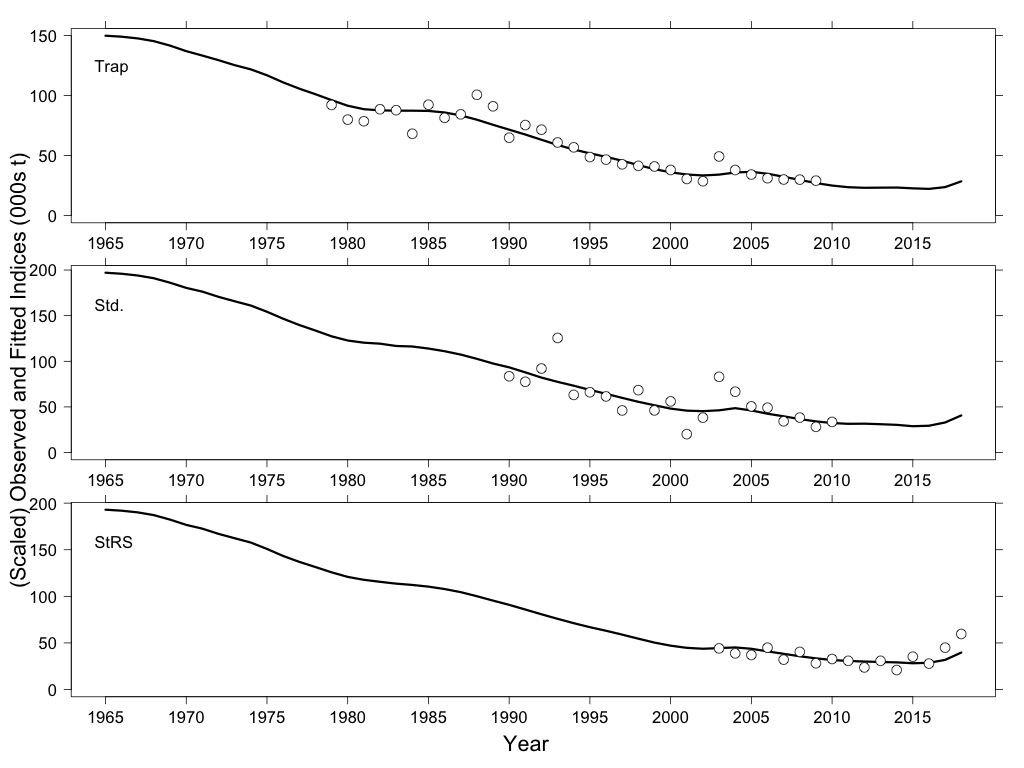
\includegraphics[width=0.9\linewidth]{data/base_ALK_mUnsexed/plotMLEindices}}{Figure \ref{fig:unnamed-chunk-13}} 

}

\caption{Operating model fits to biomass indices from the commercial trap fishery (Trap, top panel), standardized sablefish survey (Std., middle panel), and stratified random sablefish survey (StRS, bottom panel). Points show observations scaled by catchability, and lines show operating model vulnerable biomass.}\label{fig:unnamed-chunk-13}
\end{figure}
\newpage
\begin{figure}[htb]

{\centering \pdftooltip{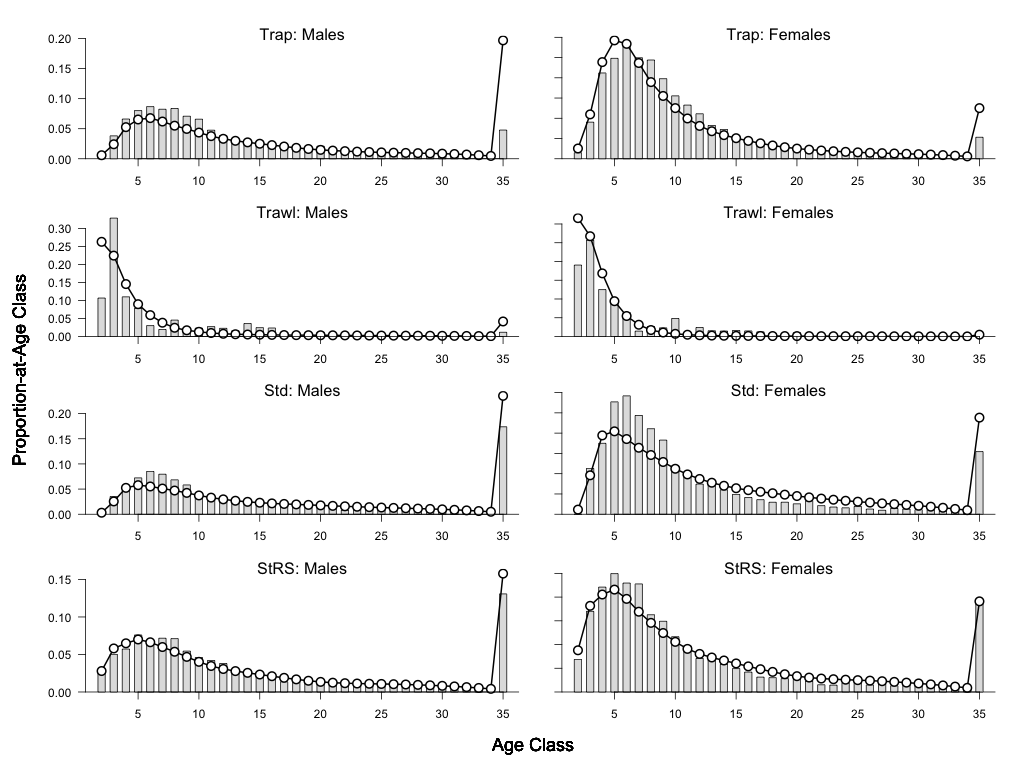
\includegraphics[width=0.9\linewidth]{data/base_ALK_mUnsexed/plotFitAgeFreq_avg}}{Figure \ref{fig:unnamed-chunk-14}} 

}

\caption{Averaged operating model fits to age observations for, from top to bottom, the commercial trap fishery (Trap), commercial trawl fishery (Trawl), standardized survey (Std.), and stratified random survey (StRS). Grey bars are the average proportion of age observations, and the points joined with a line show the average expected distribution of age observations in the operating model. Averages are taken over the years with observations.}\label{fig:unnamed-chunk-14}
\end{figure}
\newpage
\begin{figure}[htb]

{\centering \pdftooltip{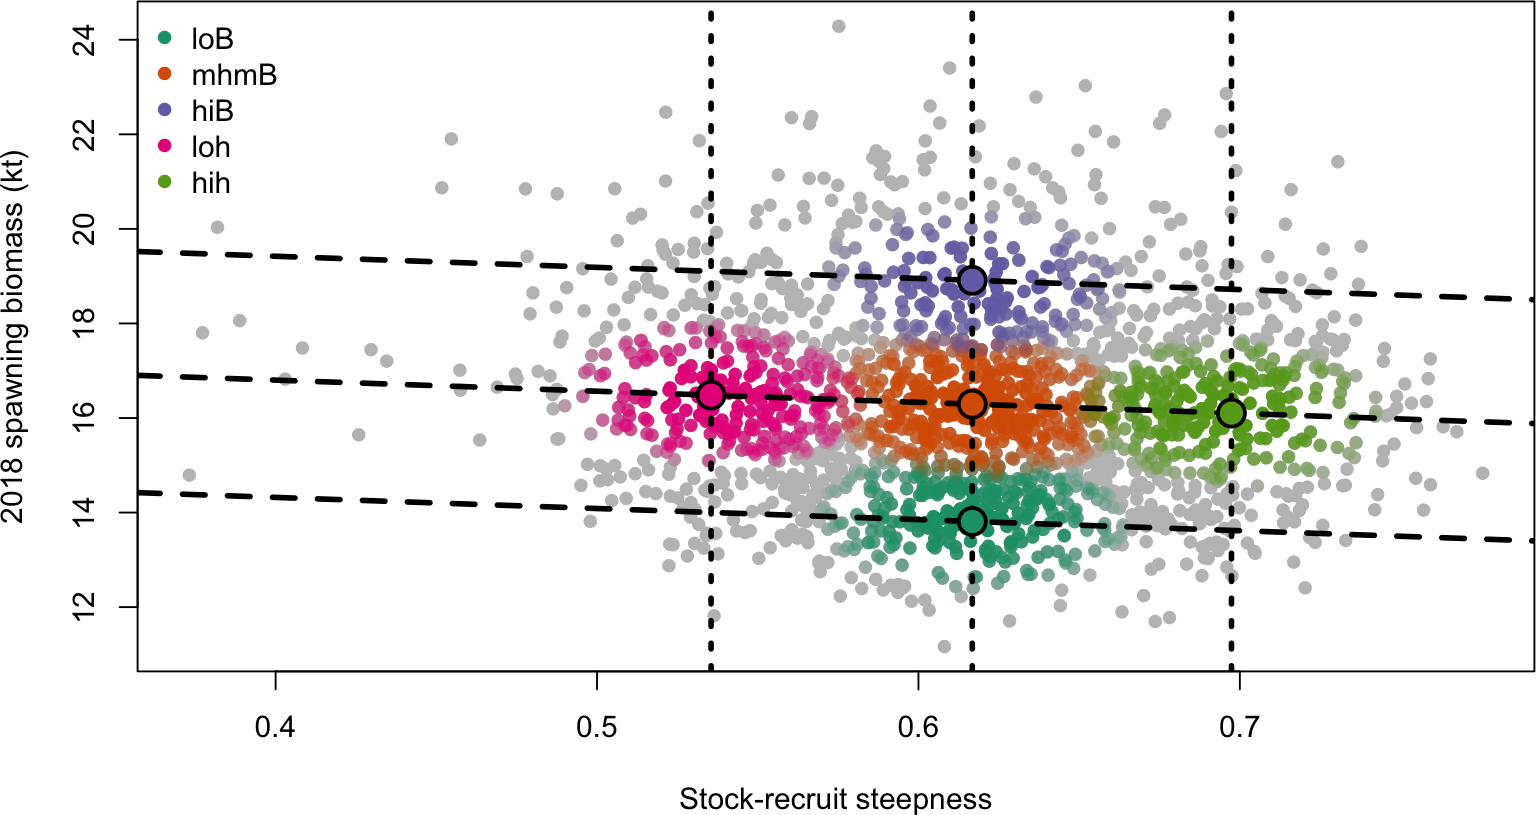
\includegraphics[width=0.9\linewidth]{knitr-figs-pdfunnamed-chunk-15-1}}{Figure \ref{fig:unnamed-chunk-15}} 

}

\caption{Joint marginal posterior distribution MCMC samples (grey dots) for stock-recruit steepness ($h$) and spawning biomass in 2018 ($B_{2018}$). Dashed lines indicate the mean, 10th and 90th percentiles of each marginal distribution, with the percentiles of the spawning biomass distribution adjusted to match the regression line between the two marginal distributions. Coloured dots with black borders at the intersections of selected percentiles are the sample centres for the 5 productivity/biomass operating model scenarios, with the coloured posterior MCMC samples showing the set of all points within a Mahalanobis distance of .6 from the centre of the same colour.}\label{fig:unnamed-chunk-15}
\end{figure}
\newpage
\begin{landscape}
\begin{figure}[htb]

{\centering \pdftooltip{\includegraphics[width=0.9\linewidth]{data/BtFitUtRt/hiRec2016_wtd/SP_hstAl_am5/BtFitUtRt_rep13}}{Figure \ref{fig:unnamed-chunk-17}} 

}

\caption{A single simulation replicate drawn from the reference set of high 2016 recruitment scenario operating models. The top row of panels show the spawning biomass and AM fits when estimated by an MP, the middle row shows the legal and sub-legal harvest rates, and the bottom row shows the OM recruitments.}\label{fig:unnamed-chunk-17}
\end{figure}
\newpage
\begin{figure}[htb]

{\centering \pdftooltip{\includegraphics[width=0.9\linewidth]{data/BtFitUtRt/simRec2016_wtd/SP_hstAl_am5/BtFitUtRt_rep13}}{Figure \ref{fig:unnamed-chunk-18}} 

}

\caption{A single simulation replicate drawn from the reference set of high 2016 recruitment scenario operating models. The top row of panels show the spawning biomass and AM fits when estimated by an MP, the middle row shows the legal and sub-legal harvest rates, and the bottom row shows the OM recruitments.}\label{fig:unnamed-chunk-18}
\end{figure}
\newpage
\begin{figure}[htb]

{\centering \pdftooltip{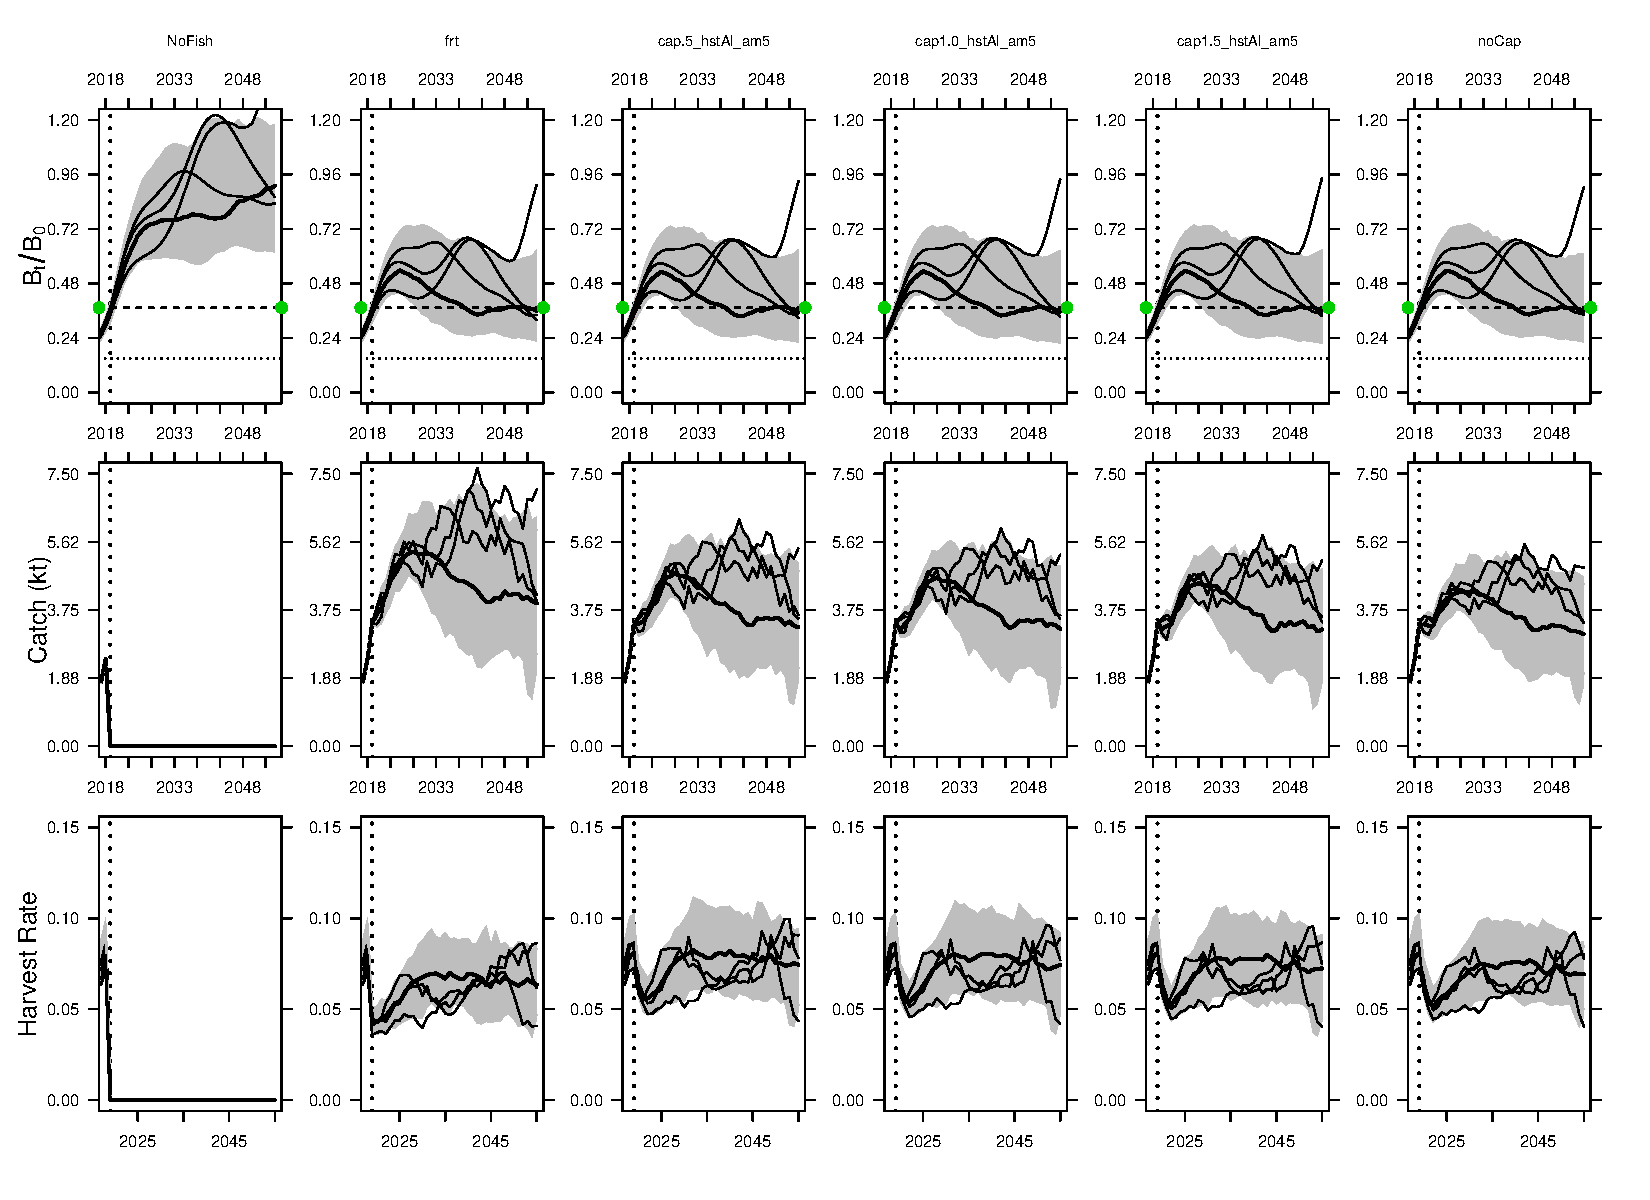
\includegraphics[width=0.9\linewidth]{data/tulipPlots/hiRec2016_wtd/depCatchHR/hiRec2016_wtd_depCatchHR_SP_hstAl_am5}}{Figure \ref{fig:unnamed-chunk-20}} 

}

\caption{Weighted combined simulation envelopes from the 5 productivity and biomass operating models in the reference recruitment scenario, showing SP management procedures that applied the historical allocation of discarding, and amortized penalties over 5 years. The top row hows projected biomass relative to unfished, the second row shows the landed catch, and the bottom row shows the legal harvest rate.}\label{fig:unnamed-chunk-20}
\end{figure}
\newpage
\begin{figure}[htb]

{\centering \pdftooltip{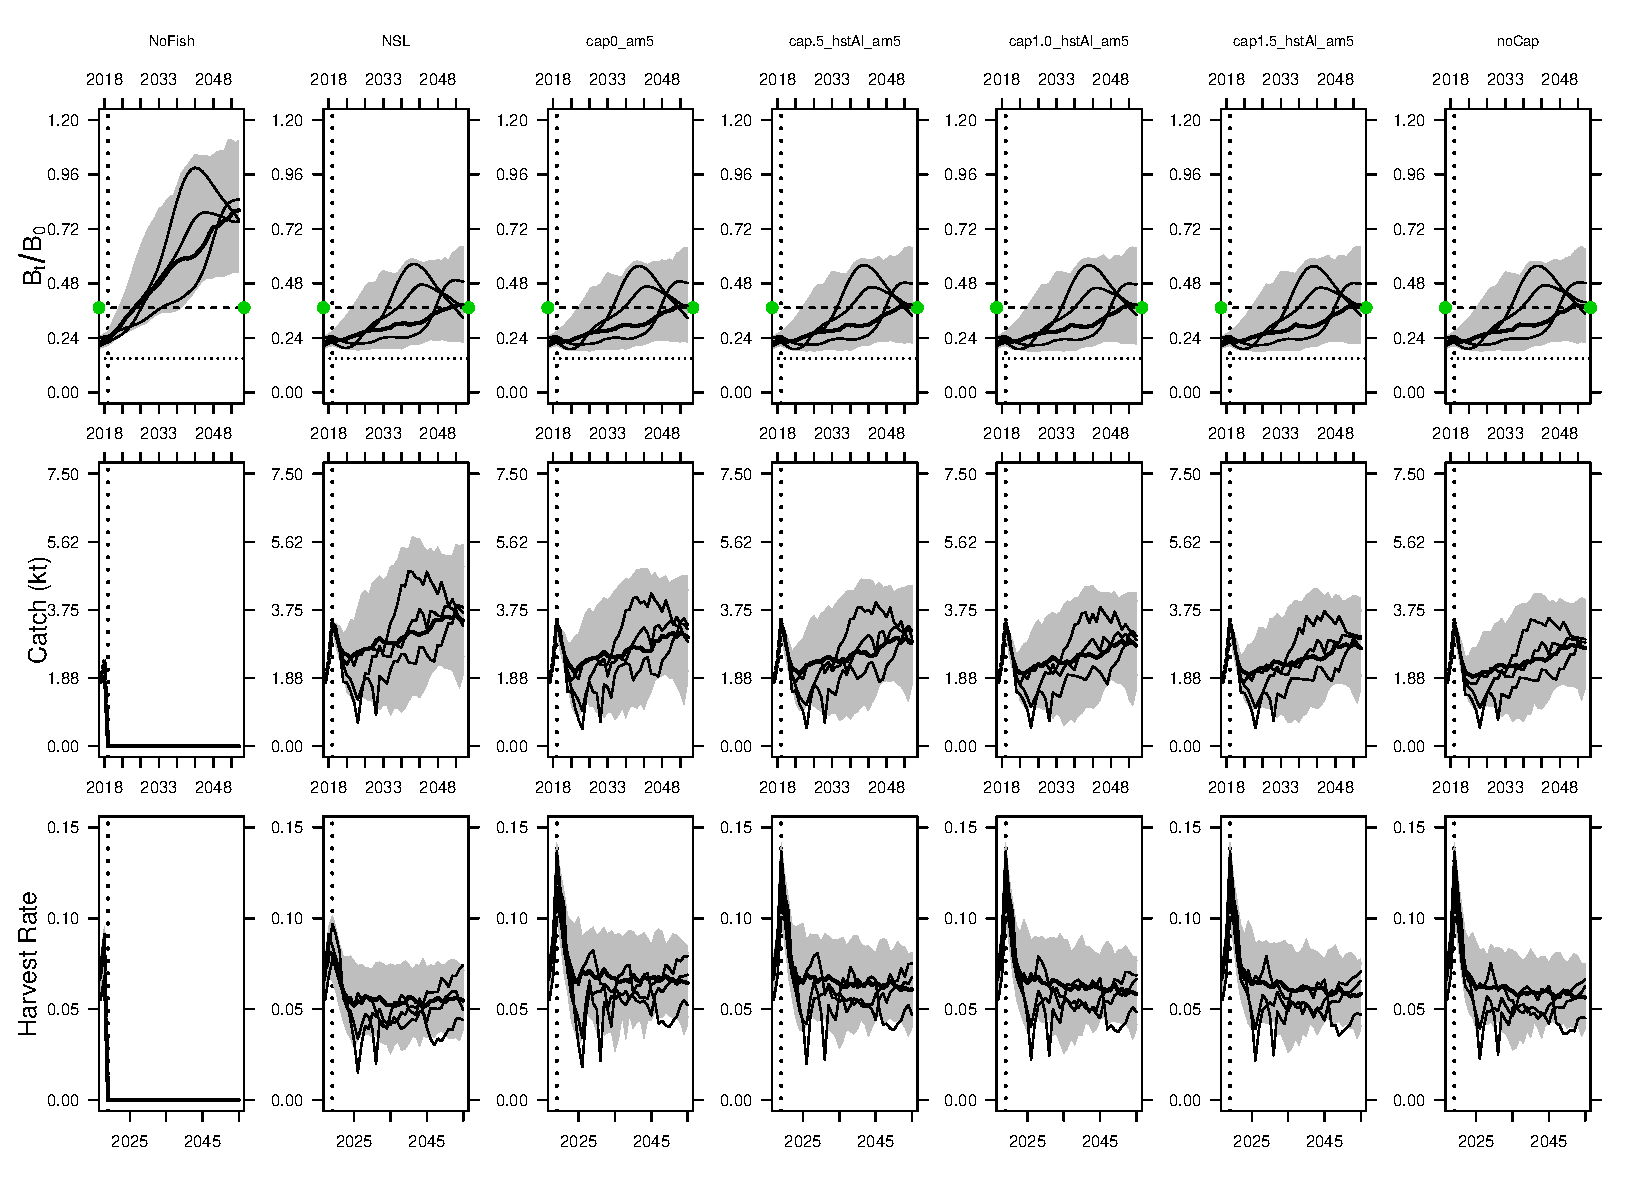
\includegraphics[width=0.9\linewidth]{data/tulipPlots/simRec2016_wtd/depCatchHR/simRec2016_wtd_depCatchHR_SP_hstAl_am5}}{Figure \ref{fig:unnamed-chunk-21}} 

}

\caption{Weighted combined simulation envelopes from the 5 productivity and biomass operating models in the robustness recruitment scenario, showing SP management procedures that applied the historical allocation of discarding, and amortized penalties over 5 years. The top row hows projected biomass relative to unfished, the second row shows the landed catch, and the bottom row shows the legal harvest rate.}\label{fig:unnamed-chunk-21}
\end{figure}
\newpage
\begin{figure}[htb]

{\centering \pdftooltip{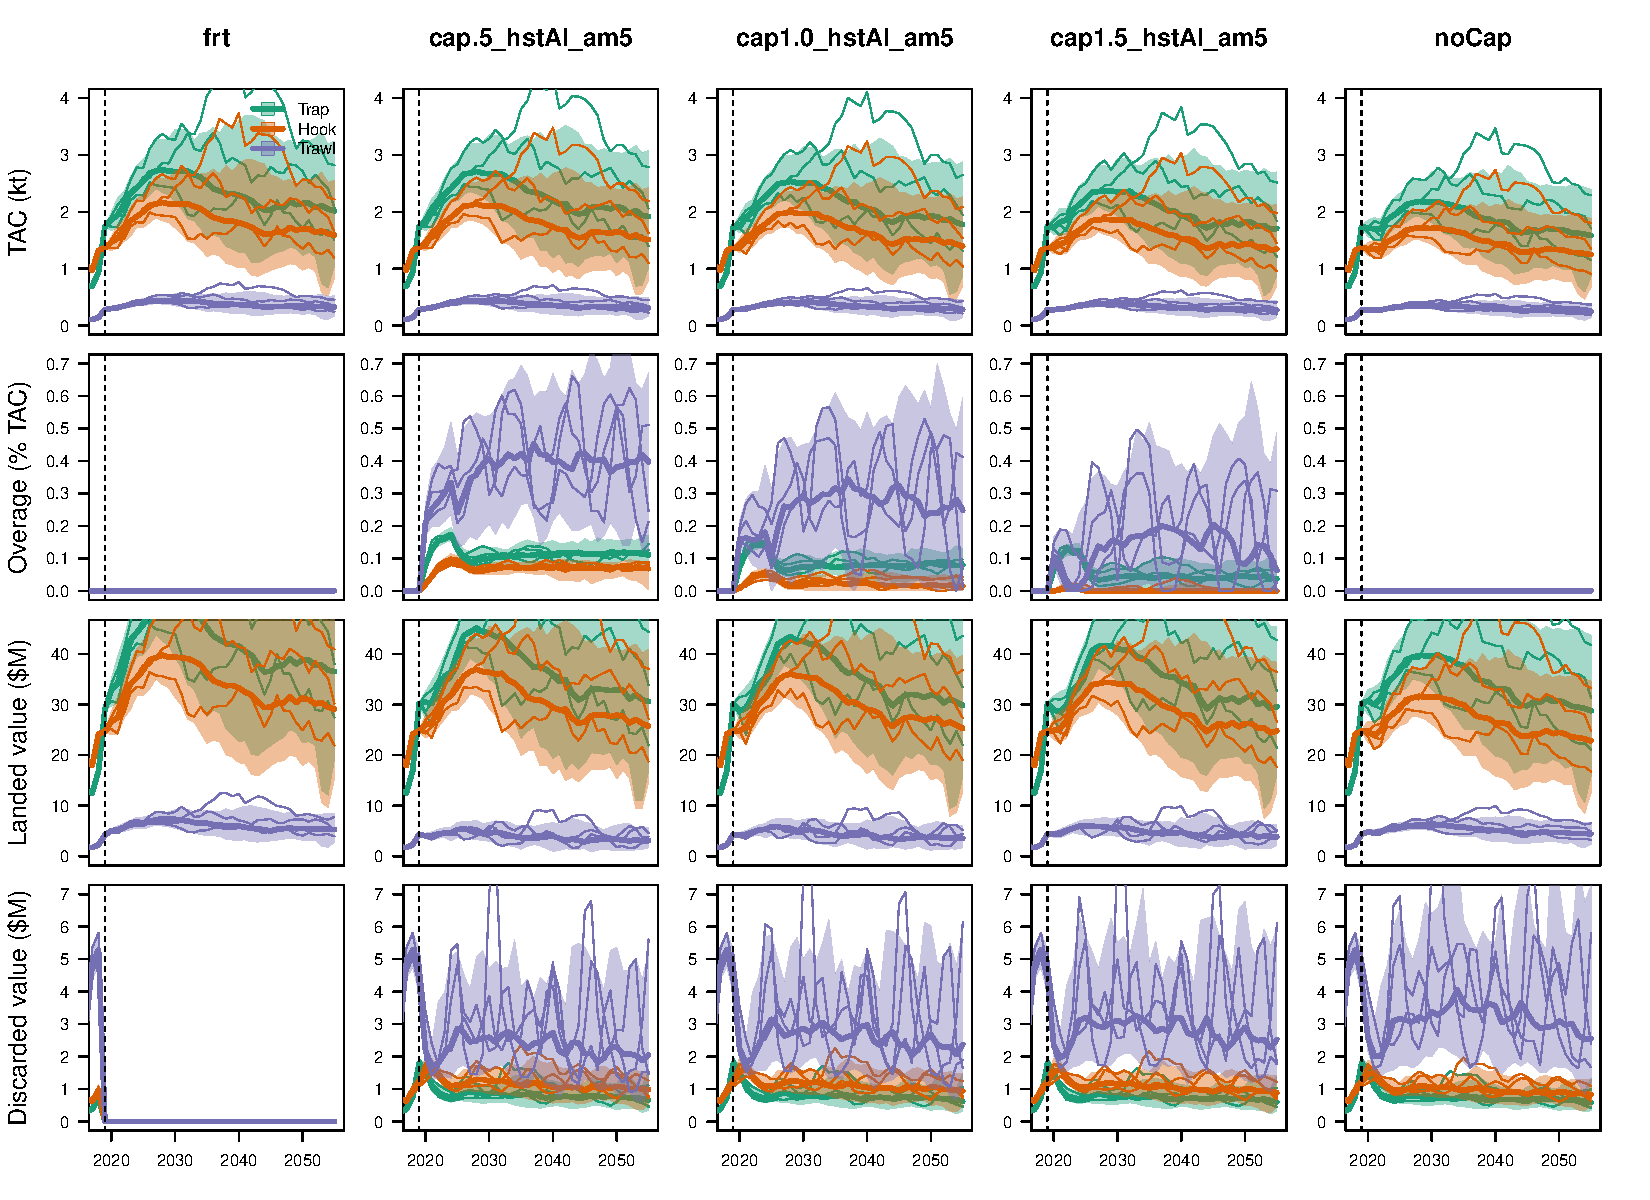
\includegraphics[width=0.9\linewidth]{data/tulipPlots/hiRec2016_wtd/TAC_overage_Val/hiRec2016_wtd_TacOverVal_SP_hstAl_am5}}{Figure \ref{fig:unnamed-chunk-23}} 

}

\caption{Simulation envelopes showing the effect of at-sea-release regulations by commercial sector under the reference recruitment scenario. Envelopes show decreasing restrictiveness of juvenile release caps from left to right. The top row shows the total available catch, the second row shows release overages as a percentage of the TAC, the third row shows the value of the landed catch, and the bottom row shows the value of released fish.}\label{fig:unnamed-chunk-23}
\end{figure}
\newpage
\begin{figure}[htb]

{\centering \pdftooltip{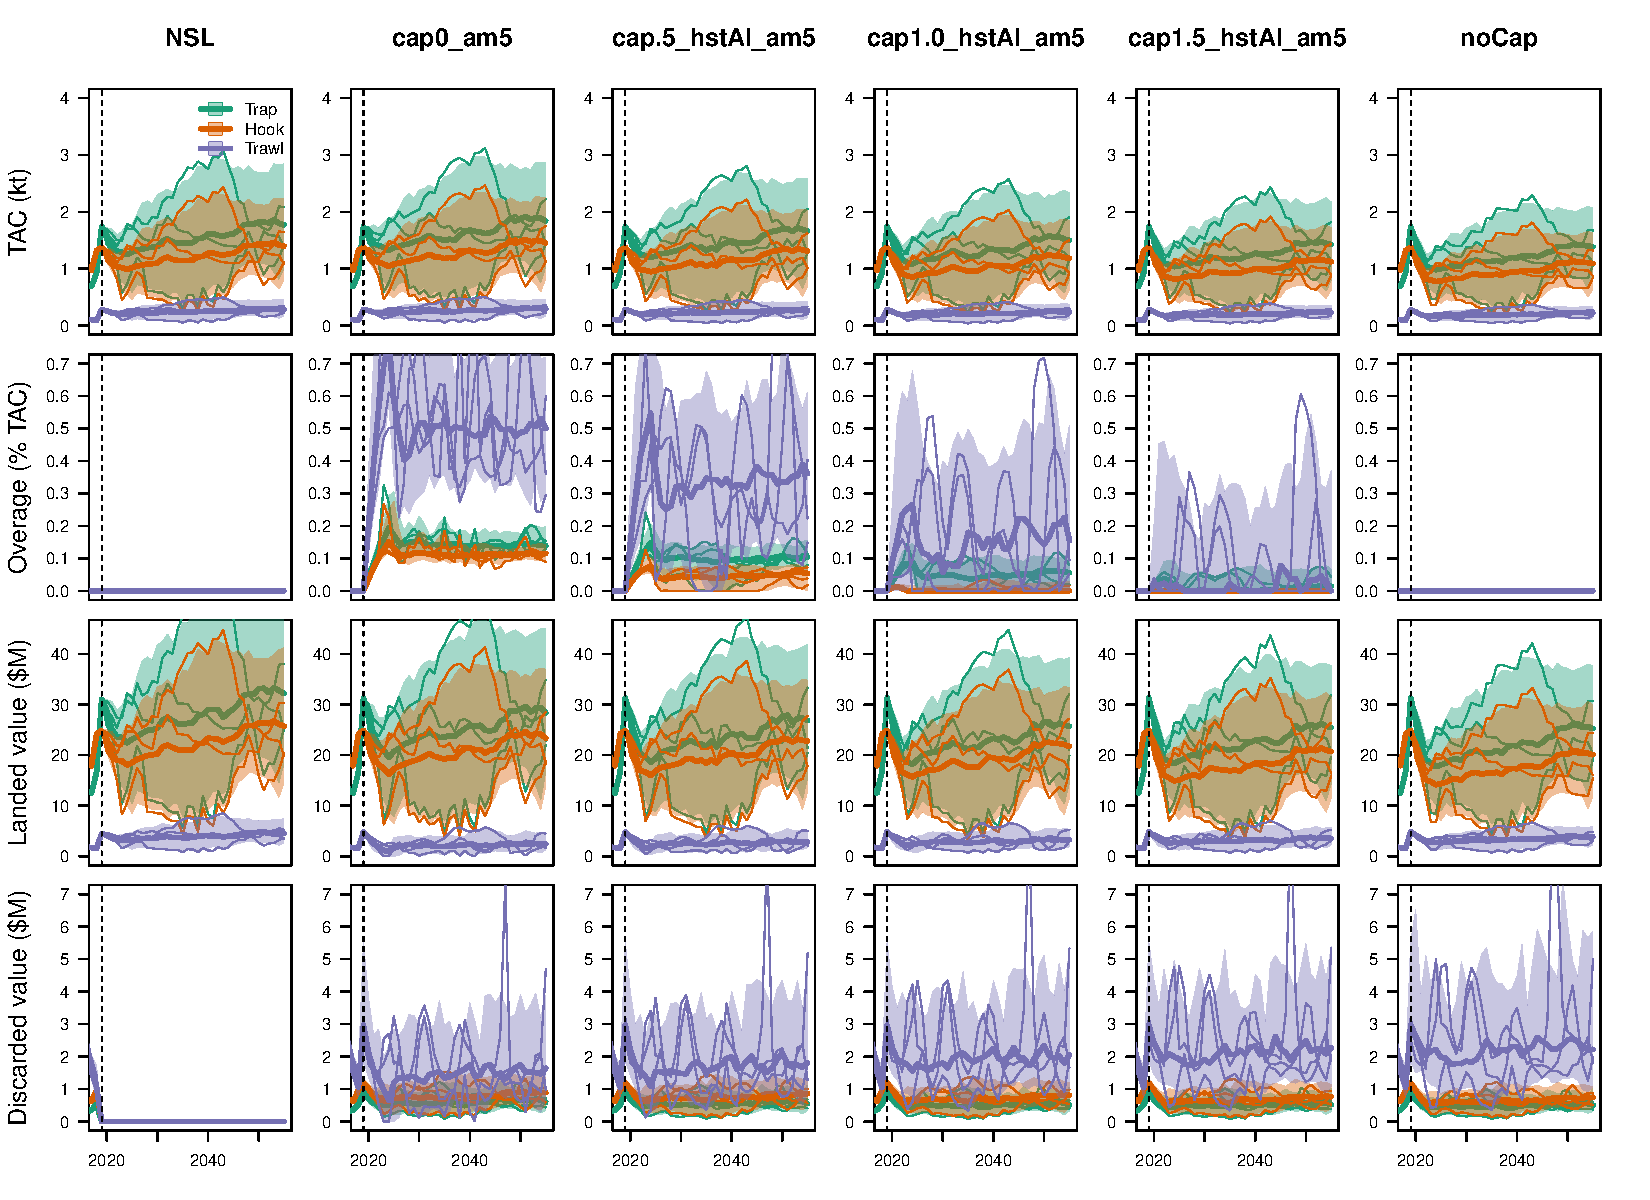
\includegraphics[width=0.9\linewidth]{data/tulipPlots/simRec2016_wtd/TAC_overage_Val/simRec2016_wtd_TacOverVal_SP_hstAl_am5}}{Figure \ref{fig:unnamed-chunk-24}} 

}

\caption{Simulation envelopes showing the effect of at-sea-release regulations by commercial sector under the robustness recruitment scenario. Envelopes show decreasing restrictiveness of juvenile release caps from left to right. The top row shows the total available catch, the second row shows release overages as a percentage of the TAC, the third row shows the value of the landed catch, and the bottom row shows the value of released fish.}\label{fig:unnamed-chunk-24}
\end{figure}
\end{landscape}
\MakeAvailable

\end{document}
